%\documentclass[a4paper, twoside, 12pt, openright]{report}
\documentclass[a4paper, twoside, 12pt]{report}

\usepackage{packages/miseEnPage}

\usepackage{vocabulaire/vocabulaire}

\usepackage[francais]{babel}
\usepackage[utf8]{inputenc}
\usepackage[T1]{fontenc}
\usepackage{graphicx}
\usepackage{fancyhdr}
\usepackage{pdfpages}
\usepackage{float}
\usepackage{diagbox}
\usepackage[urlcolor=blue, linkcolor=black,linktoc=all, colorlinks=true]{hyperref}
\usepackage[left=2.5cm, right=2.5cm, top=2.5cm, bottom=2.5cm, headheight=15pt]{geometry}
\usepackage[final]{pdfpages}
\usepackage{helvet}
\usepackage{lscape}
\renewcommand{\familydefault}{\sfdefault}

\makeatletter
\def\@makechapterhead#1{% chapter
  \vspace*{5\p@}
  {
    \parindent \z@ \raggedright \normalfont
    \ifnum \c@secnumdepth >\m@ne
    \huge\bfseries \@chapapp\space \thechapter
    \par\nobreak
    \vskip 5\p@
    \fi
    \interlinepenalty\@M
    \Huge \bfseries #1\par\nobreak
    \vskip 10\p@
    \thispagestyle{fancy}% Permet d'ajouter l'entête de pied de page
  }
}

\def\@schapter#1{
  \if@twocolumn
  \@topnewpage[\@makeschapterhead{#1}]
  \else
  \@makeschapterhead{#1}
  \@afterheading
  \fi
}

\def\@makeschapterhead#1{% chapter*
  \vspace*{5\p@}
  {
    \parindent \z@ \raggedright
    \normalfont
    \interlinepenalty\@M
    \Huge \bfseries  #1\par\nobreak
    \vskip 10\p@
    \thispagestyle{fancy} % Permet d'ajouter l'entête de pied de page
  }
}
\makeatother


%\usepackage[francais]{babel}
\usepackage[utf8]{inputenc}
\usepackage[T1]{fontenc}
\usepackage{graphicx}
\usepackage{fancyhdr}
\usepackage{pdfpages}
\usepackage{float}
\usepackage{diagbox}
\usepackage[urlcolor=blue, linkcolor=black,linktoc=all, colorlinks=true]{hyperref}
\usepackage[left=2.5cm, right=2.5cm, top=2.5cm, bottom=2.5cm, headheight=15pt]{geometry}
\usepackage[final]{pdfpages}
\usepackage{helvet}
\usepackage{lscape}
\renewcommand{\familydefault}{\sfdefault}

\makeatletter
\def\@makechapterhead#1{% chapter
  \vspace*{5\p@}
  {
    \parindent \z@ \raggedright \normalfont
    \ifnum \c@secnumdepth >\m@ne
    \huge\bfseries \@chapapp\space \thechapter
    \par\nobreak
    \vskip 5\p@
    \fi
    \interlinepenalty\@M
    \Huge \bfseries #1\par\nobreak
    \vskip 10\p@
    \thispagestyle{fancy}% Permet d'ajouter l'entête de pied de page
  }
}

\def\@schapter#1{
  \if@twocolumn
  \@topnewpage[\@makeschapterhead{#1}]
  \else
  \@makeschapterhead{#1}
  \@afterheading
  \fi
}

\def\@makeschapterhead#1{% chapter*
  \vspace*{5\p@}
  {
    \parindent \z@ \raggedright
    \normalfont
    \interlinepenalty\@M
    \Huge \bfseries  #1\par\nobreak
    \vskip 10\p@
    \thispagestyle{fancy} % Permet d'ajouter l'entête de pied de page
  }
}
\makeatother


% Paramètres de la page de garde

\titreAcronyme{Traitement d'Image \newline Jérôme \bsc{Desseaux} \& Pierre-Alain \bsc{Emo} \& Clément \bsc{Gomme}}
\titreGeneral{Detection, segmentation and classification of 3D urban
objects using mathematical morphology and supervised
learning}
\titreDetaille{Rapport}
\version{1.00}

% Renseignements sur le document

\auteurs{\jerome \newline \pa \clement}
\resume{Ce document présente le plan de gestion des configuration du PIC \nomPic{}}

\referenceVersion{V1.00}

\begin{document}

\couverture{}

%\input{src/\nomPic_Q_PGC_Partie01}

\newpage

\begin{abstract}
Harum trium sententiarum nulli prorsus assentior. Nec enim illa prima vera est, ut, quem ad modum in se quisque sit, sic in amicum sit animatus. Quam multa enim, quae nostra causa numquam faceremus, facimus causa amicorum! precari ab indigno, supplicare, tum acerbius in aliquem invehi insectarique vehementius, quae in nostris rebus non satis honeste, in amicorum fiunt honestissime; multaeque res sunt in quibus de suis commodis viri boni multa detrahunt detrahique patiuntur, ut iis amici potius quam ipsi fruantur.

\end{abstract}

\pagestyle{pageNormale}
\setcounter{page}{1}

\tableofcontents{}

\newpage

%%%%%%%%%%%%%%%%%%%%%%%%%%%%%%%%%%%%%%%%%%%%
%    Inclure les différentes parties du    %
%   ici. ex : \input{src/nom_du_fichier}   %
%%%%%%%%%%%%%%%%%%%%%%%%%%%%%%%%%%%%%%%%%%%%

%\input{src/02_userstories}
\chapter{Introduction}

\chapter{Travaux relatifs}

\chapter{Méthodologie}

\begin{figure}[H]
\centering
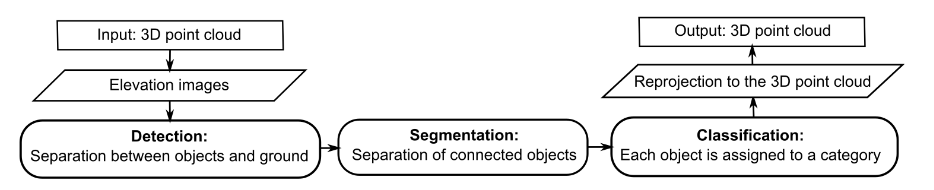
\includegraphics[width=0.9\linewidth]{./images/methodo.png}
\caption{Schéma montrant les différentes étapes du processus de modélisation du nuage 3D}
\end{figure}

\paragraph{Elévation :} Le nuage de point 3D est projeté sur des images d’élévation.

\paragraph{Détection :}Un DTM [Digital Terrain Model] ou MNE [Modèle Numérique d’Elévation] en français, est automatiquement créé et les objets hypothétique sont générés comme des discontinuités sur le sol.

\paragraph{Segmentation :} Les facades sont segmentées automatiquement comme les structures verticales les plus hautes sur les images d’élévation. Ensuite les petites régions isolées sont éliminées, et les objets connectés sont segmentés. Le résultat de l’étape de segmentation crée une image d’étiquettes, où chaque objet segmenté contient un identifiant unique.

\paragraph{Classification :} Par la suite, de nombreuses caractéristiques géométriques sont calculées et un classement est opéré. A partir de l’étape de classement, une image de classes est crée, contenant une catégorie pour chaque objet segmenté. 
Le fait d’avoir les étiquettes et les classes dans deux images différentes est utile dans le cas des objets connectés appartenant à la même classe (par exemple un alignement de voiture garées). 
Reprojection : Finalement, les images de classes et d’étiquettes sont reprojetées sur le nuage de points 3D afin d’obtenir le résultat final. Cette étape transforme les images 2D en nuage de points 3D. Chaque pixel du nuage de point prend l’étiquette et la classe de ce pixel.

\section{Images d'élévation}

Les images d’élévation sont des structures en $2.5D$ qui contiennent une information sur l’altitude de chaque pixel. Les nuages de points 3D sont projetés sur des images d’élévation car elles sont des structures pratiques pour visualiser et traiter les données. On peut utiliser tous les outils de traitements d’image existants, en particulier la morphologie mathématique (Mathero, 1975; Serra; 1988; Soille, 2003). De plus, les images peuvent être traitées rapidement, implicitement définissent les relations de voisinage, et requière moins de mémoire que les données 3D.

Les images d’élévation sont générées par une \textbf{projection orthographique} du nuage de points 3D en utilisant une caméra virtuelle. La caméra virtuelle est placée sur le plan horizontal et croise le point le plus bas dans le nuage de point $(0, 0, z_{min})$. Par conséquent, chaque pixel de l’image d’élévation contient l’élévation de la cellule de grille au dessus de $z_{min}$. Le seul paramètre libre dans cette projection est la taille du pixel spatial, qui doit être choisi avec attention. 
\begin{itemize}
\item Si il est trop large, trop de points seront projetés sur le même pixel, faisant ainsi perdre les détails. 
\item Si il est trop petit, cela implique des problèmes de connectivité et des grandes tailles d’images, ce qui ne justifierait plus l’utilisation d’images d’élévation à la place des nuages de points 3D. 
\end{itemize}

\vspace{1em}

Pour éviter les problèmes de connectivité et la parte d’information, la taille du pixel spatial est choisi selon la résolution du nuage de points.
En général, de nombreux points sont projetés sur le même pixel. Par conséquent, quatres images sont définies :

\begin{enumerate}
\item Image d’élévation maximum (ou simplement image d’élévation), stocke l’élévation maximale entre tous les points projetés sur le même pixel ;
\item Image d’élévation minimal, stocke l’élévation minimum entre tous les points projetés sur le même pixel ;
\item Image de différence de hauteurs, contient la différence entre les deux images précédentes ;
\item Image d’accumulation, qui stocke le nombre de points projetés sur chaque pixel.
\end{enumerate}

\vspace{1em}

En général, les étapes opératoires sont effectuées sur l’image d’élévation maximum. Les autres images sont utilisées pour supporter certaines décisions lors des analyses ou pour traiter les caractéristiques des objets.
Après la création de l’image, une interpolation morphologique est effectuée afin de remplir les trous causés par les occlusions et les lignes de balayage manquantes. Une technique d’interpolation basée sur l’opération morphologique \enquote{fill holes} est préférée puisque cette transformation ne crée pas un nouveau maximum de région dans l’image. Un trou est une région sombre (= entourée par des pixels plus clairs), non connectée au bord de l’image. Cette méthode d’interpolation a été proposé par Hernandez and Marcotegui (2009a) et une explication détaillée peut être trouvée dans Serna and Marcotegui, 2013b.

Quand la détection, la segmentation et la classification ont été effectuées, les images sont projetées sur le nuage de points 3D. 

\section{Détection}

\section{Segmentation}
\subsection{Sol}
\subsection{Objets}


\section{Classification}
\chapter{Résultats}

\chapter{Conclusion}



\pageQuatriemeCouverture{}

\end{document}
